\documentclass[12pt,]{article}
\usepackage{lmodern}
\usepackage{amssymb,amsmath}
\usepackage{ifxetex,ifluatex}
\usepackage{fixltx2e} % provides \textsubscript
\ifnum 0\ifxetex 1\fi\ifluatex 1\fi=0 % if pdftex
  \usepackage[T1]{fontenc}
  \usepackage[utf8]{inputenc}
\else % if luatex or xelatex
  \ifxetex
    \usepackage{mathspec}
    \usepackage{xltxtra,xunicode}
  \else
    \usepackage{fontspec}
  \fi
  \defaultfontfeatures{Mapping=tex-text,Scale=MatchLowercase}
  \newcommand{\euro}{€}
    \setmainfont{Georgia}
\fi
% use upquote if available, for straight quotes in verbatim environments
\IfFileExists{upquote.sty}{\usepackage{upquote}}{}
% use microtype if available
\IfFileExists{microtype.sty}{%
\usepackage{microtype}
\UseMicrotypeSet[protrusion]{basicmath} % disable protrusion for tt fonts
}{}
\usepackage[margin=1in]{geometry}
\ifxetex
  \usepackage[setpagesize=false, % page size defined by xetex
              unicode=false, % unicode breaks when used with xetex
              xetex]{hyperref}
\else
  \usepackage[unicode=true]{hyperref}
\fi
\hypersetup{breaklinks=true,
            bookmarks=true,
            pdfauthor={},
            pdftitle={},
            colorlinks=true,
            citecolor=blue,
            urlcolor=blue,
            linkcolor=magenta,
            pdfborder={0 0 0}}
\urlstyle{same}  % don't use monospace font for urls
\usepackage{graphicx,grffile}
\makeatletter
\def\maxwidth{\ifdim\Gin@nat@width>\linewidth\linewidth\else\Gin@nat@width\fi}
\def\maxheight{\ifdim\Gin@nat@height>\textheight\textheight\else\Gin@nat@height\fi}
\makeatother
% Scale images if necessary, so that they will not overflow the page
% margins by default, and it is still possible to overwrite the defaults
% using explicit options in \includegraphics[width, height, ...]{}
\setkeys{Gin}{width=\maxwidth,height=\maxheight,keepaspectratio}
\setlength{\parindent}{0pt}
\setlength{\parskip}{6pt plus 2pt minus 1pt}
\setlength{\emergencystretch}{3em}  % prevent overfull lines
\providecommand{\tightlist}{%
  \setlength{\itemsep}{0pt}\setlength{\parskip}{0pt}}
\setcounter{secnumdepth}{0}

%%% Use protect on footnotes to avoid problems with footnotes in titles
\let\rmarkdownfootnote\footnote%
\def\footnote{\protect\rmarkdownfootnote}

%%% Change title format to be more compact
\usepackage{titling}

% Create subtitle command for use in maketitle
\newcommand{\subtitle}[1]{
  \posttitle{
    \begin{center}\large#1\end{center}
    }
}

\setlength{\droptitle}{-2em}
  \title{}
  \pretitle{\vspace{\droptitle}}
  \posttitle{}
  \author{}
  \preauthor{}\postauthor{}
  \date{}
  \predate{}\postdate{}

\usepackage{booktabs}
\usepackage[final]{changes}
\usepackage[font={small},labelfont=bf,labelsep=colon]{caption}
\linespread{1.2}
\usepackage[compact]{titlesec}
\usepackage{enumitem}
\usepackage{tikz}
\def\checkmark{\tikz\fill[scale=0.4](0,.35) -- (.25,0) -- (1,.7) -- (.25,.15) -- cycle;}
\setlist{nolistsep}
\titlespacing{\section}{2pt}{*0}{*0}
\titlespacing{\subsection}{2pt}{*0}{*0}
\titlespacing{\subsubsection}{2pt}{*0}{*0}
\setlength{\parskip}{3pt}
\setremarkmarkup{(#2)}

% Redefines (sub)paragraphs to behave more like sections
\ifx\paragraph\undefined\else
\let\oldparagraph\paragraph
\renewcommand{\paragraph}[1]{\oldparagraph{#1}\mbox{}}
\fi
\ifx\subparagraph\undefined\else
\let\oldsubparagraph\subparagraph
\renewcommand{\subparagraph}[1]{\oldsubparagraph{#1}\mbox{}}
\fi

\begin{document}
\maketitle

\section{Response to reviewers}\label{response-to-reviewers}

\emph{\textcolor{blue}{We appreciate the time spent by the editors and reviewers in
assessing our manuscript.  Please see below for a point-by-point response to the
issues raised.}}

\subsection{Reviewer 1}\label{reviewer-1}

Thank you for the opportunity to review the paper ``Supervised learning
technique for the automated identification of white matter
hyperintensities in traumatic brain injury''. In this study, the authors
present a machine learning algorithm for automated segmentation of white
matter hyperintensities, a form of white matter degeneration visible in
FLAIR-MRI that is observed in a wide range of clinical syndromes, and
even in healthy controls. The method proposed by the authors relies on
training random forests to learn the relationship between voxel
intensities in a set of feature images derived from multimodal MRI (T1,
T2, FLAIR) and lesions drawn manually by an expert. Since the method
uses examples to learn what constitutes a lesion, this is correctly
considered a supervised method. The method is applied on a set of 24
patients with clinically confirmed traumatic brain injury, and results
are obtained with a leave-one-out cross validation.

Overall, the method proposed by the authors is innovative and
thoughtful, and has great potential for bridging the gap between
research findings and clinical needs. The method uses a series of
cutting edge solutions to the segmentation problem: (1) multimodal
imaging inputs, which is known to increase segmentation accuracy, (2)
random forests, which are an excellent tool for finding multivariate
nonlinear relationships, (3) voxel neighborhood information, which
provide contextual information for each voxel, and (4) an algorithm that
improves the segmentation in stages. However, the manuscript itself, to
my opinion, is not well focused and needs significant improvement. Below
are my specific comments in support of this.

\begin{quote}
\emph{\textcolor{blue}{We thank the reviewer for the generally positive assessment of our work.  We also
appreciate the detailed critique below to help us improve specific aspects of the
presentation.}}
\end{quote}

Major comments:

\begin{enumerate}
\def\labelenumi{\arabic{enumi}.}
\tightlist
\item
  The biggest issue I had while reading the manuscript is the lack of a
  coherent theme of what this paper is about. The authors span their
  exposé from multiple sclerosis to the automobile industry, without
  stating why these links to other diseases (or industries) have any
  relevance. It appears in some parts that the closest disease with
  similar white matter lesions is multiple sclerosis, but this is not
  clearly stated, nor the two types of lesions are compared. It is,
  therefore, unclear why counting how many MS lesion segmentation
  methods are publicly available is of any importance. When explaining
  methods, the authors mention the utility of support vector machines,
  or the existence of a python package called SciPy. Yet, it is unclear
  why these things have any importance, unless the authors make
  connections to their topic/method.
\end{enumerate}

\begin{quote}
\emph{\textcolor{blue}{We reduced the introduction to limit the clinical motivation to a
TBI context and removed mention of multiple sclerosis to remove any assumption of
disease similarity (although the segmentation approaches can be similar).  We also
removed the paragraph dealing with publicly available software for neuroimaging analysis.
}}
\end{quote}

\begin{enumerate}
\def\labelenumi{\arabic{enumi}.}
\setcounter{enumi}{1}
\tightlist
\item
  Second, the manuscript has no results. All the results section is
  focused on talking about feature ranking, which by the way is
  explained in the Results section instead of the Methods section. The
  most important results (the prediction accuracy of automated
  segmentation), are not mentioned in the manuscript but are only
  plotted in Figure 7. My advice is to put the focus of the results
  section on accuracy, i.e., give precise dice values and perhaps add
  other measures (metric displacement, Hausdorf distance, sensitivity,
  specificity, etc.). Also, the gain in accuracy from stage 1 to stage 2
  cannot be guessed by looking at a plot, the authors must provide a
  statistical comparison. When investigating accuracy, the error in
  lesion size should be reported, both in terms of volume and in terms
  of individual lesions counts (i.e.~out of 10 lesions 9 were found, 1
  was missed, etc.). This information is crucial to clinicians, if the
  authors foresee the use of the method in a clinical setting, as it
  seems from the discussion. Beside adding results to the manuscript, it
  is equally important to give some results in the abstract. The
  abstract must be self-sufficient in reporting all the major points of
  the paper.
\end{enumerate}

\begin{quote}
\emph{\textcolor{blue}{We completely reorganized the results and discussion
section to reflect the new evaluation.  In addition, we added a synopsis
of these results to the abstract.}}
\end{quote}

\begin{enumerate}
\def\labelenumi{\arabic{enumi}.}
\setcounter{enumi}{2}
\tightlist
\item
  Third, there is no information about the manual lesion tracing
  procedure. Were lesion drawn on FLAIR or were other modalities used as
  well? If FLAIR was used as reference it is not surprising that FLAIR
  emerges as one of the top predictive modalities.
\end{enumerate}

\begin{quote}
\emph{\textcolor{blue}{We added the following to the Methods section:}}
\end{quote}

\begin{quote}
\textcolor{blue}{The first author (J. R. S.) performed the manual WMH tracings for all 26  subjects.  J. R. S. is a radiologist certified by the American Board of Radiology, with a certificate of advanced qualification in vascular and interventional radiology, over 18 years of research experience in TBI, and 6 years of clinical imaging experience.  All multi-modal MR dicom image slices were converted to the nifti file format. All nifti image volumes for each subject were rigidly aligned to the T1 image of that subject using the ANTs software}\textsuperscript{1}
\textcolor{blue}{.  The normalized MRI volumes were then provided to J. R. S. who traced each lesion using the ITK-SNAP tool}\textsuperscript{2}
\textcolor{blue}{ which has multi-image overlay capabilities for visualizing all modalities in all three canonical views.}
\end{quote}

\begin{quote}
Descriptive statistics on the lesions are also necessary: how big were
the lesions, how many lesions were found in each patient (the range 1-20
is not sufficiently informative), where were the lesions located? This
information helps understand why, for example, brain stem or cerebellum
labels were not that important for achieving good lesion predictions.
\end{quote}

\begin{quote}
\emph{\textcolor{blue}{We added the following sentence to the opening paragraph of the
Imaging subsection of the Methods section:}}
\end{quote}

\begin{quote}
\textcolor{blue}{All lesions were isolated in the white matter of the cerebrum.
Table 1 provides a descriptive statistical summary of the variation in lesion load across the selected cohort.}
\end{quote}

\begin{quote}
\emph{\textcolor{blue}{as well as the corresponding table:}}
\end{quote}

\begin{table}[!htb]
  \centering
  \begin{tabular*}{1.0\textwidth}{@{\extracolsep{\fill}} rrrrr}
    \textbf{Subject id} & \textbf{Lesion count} & \textbf{Lesion load} & \textbf{Mean volume} & \textbf{[Min $-$ Max]} \\
    \toprule
    \midrule
    0 & 2 & 18 & 9 $\pm$ 1.4 & [8-10] \\
    1 & 3 & 3 & 1 $\pm$ 0 & [1-1] \\
    2 & 0 & 0 & 0 & [0-0] \\
    3 & 11 & 209 & 19 $\pm$ 18.4 & [1-56] \\
    4 & 3 & 130 & 43.3 $\pm$ 50.0 & [12-101] \\
    5 & 1 & 2 & 2 & [2-2] \\
    6 & 25 & 790 & 31.6 $\pm$ 29.2 & [2-132] \\
    7 & 24 & 767 & 32.0 $\pm$ 33.6 & [2-166] \\
    8 & 3 & 18 & 6 $\pm$ 7.8 & [1-15] \\
    9 & 21 & 508 & 24.2 $\pm$ 35.1 & [1-166] \\
    10 & 2 & 17 & 8.5 $\pm$ 10.6 & [1-16] \\
    11 & 7 & 151 & 21.6 $\pm$ 21.7 & [1-61] \\
    12 & 46 & 901 & 19.6 $\pm$ 17.9 & [1-115] \\
    13 & 1 & 1 & 1 & [1-1] \\
    14 & 2 & 32 & 16 $\pm$ 9.9 & [9-23] \\
    15 & 2 & 22 & 11 $\pm$ 14.1 & [1-21] \\
    16 & 8 & 124 & 15.5 $\pm$ 8.4 & [6-34] \\
    17 & 3 & 140 & 46.7 $\pm$ 53.1 & [1-105] \\
    18 & 3 & 10 & 3.3 $\pm$ 4.0 & [1-8] \\
    19 & 20 & 784 & 39.2 $\pm$ 63.2 & [1-230] \\
    20 & 3 & 6 & 2 $\pm$ 1.7 & [1-4] \\
    21 & 7 & 244 & 34.9 $\pm$ 32.3 & [1-93] \\
    22 & 12 & 236 & 19.7 $\pm$ 13.5 & [1-52] \\
    23 & 63 & 4078 & 64.7 $\pm$ 93.6 & [1-551] \\
    \midrule
    Total & 272 & 9191 & 33.8 $\pm$ 55.4 & [1-551] \\
    \midrule
    \bottomrule
  \end{tabular*}
\label{table:trainingData}
\caption{Descriptive lesion statistics for the cohort used for the evaluation.
         Lesion load, mean volume ($\pm$ standard deviation), and the min/max range are given in terms of
         the number of voxels
         since all image acquisitions were performed with the same image
         voxel resolution ($1\times1\times1.2$ mm$^3$).
         }
\end{table}


\clearpage

\begin{enumerate}
\def\labelenumi{\arabic{enumi}.}
\setcounter{enumi}{3}
\tightlist
\item
  Fourth, although the authors claim the method is available, I couldn't
  find any link for the public. Note, it would be equally important if
  the publication of the method online is associated with proper
  documentation on how a new (naive) user can apply it.
\end{enumerate}

\begin{quote}
\emph{\textcolor{blue}{Our methodological publication history demonstrates that we are
very supportive of open science and have released both code and data in conjunction
with these publications in public forums, such as github.  However, permission to
publicly release the data for this data has not yet been obtained and so we removed
the mention of public availability.  However, when we do get permission, it will
be posted to the github repository associated with this manuscript
(https://github.com/ntustison/WatchMeHyperventilate), which we mention in the text,
for future readers.
}}
\end{quote}

Minor comments:

\begin{enumerate}
\def\labelenumi{\arabic{enumi}.}
\setcounter{enumi}{4}
\tightlist
\item
  In the abstract, the authors mention the creation of tailored features
  for segmenting WMHs. My understanding is that the method proposed by
  the authors has no tailoring (if we think of tailoring as custom
  cutting to WMH needs).
\end{enumerate}

\begin{quote}
\emph{\textcolor{blue}{We removed the word ``tailor'' in its various forms in the
manuscript to avoid the misreading described by the reviewer.}}
\end{quote}

\begin{quote}
There was no feature selection process all the features were included as
predictors.
\end{quote}

\begin{quote}
\emph{\textcolor{blue}{Although feature selection is mentioned in the manuscript, nowhere
do we mention or imply any type of computational feature selection.  There was
a feature selection process in that we selected ones from the myriad feature images that
one can possibly produce based on our targeted application, i.e. WMHs.}}
\end{quote}

\begin{quote}
A similar pitfall if found on pg. 6 ln 56, where the manuscript reads
``Crucial to these supervised segmentation approaches are the creation
and selection of features as input in conjunction with expertly
identified structures.'' What are the structures identified by the
expert in this study?
\end{quote}

\begin{quote}
\emph{\textcolor{blue}{For this particular application, white matter hyperintensities
are the structure of interest.  We have re-emphasized this point by writing:
}}
\end{quote}

\begin{quote}
\textcolor{blue}{Crucial to these supervised segmentation approaches are the creation and selection of
``features'' as input (i.e., feature images constructed from the training data)
in conjunction with expertly identified structures of interest
(i.e., WMHs) for model construction.}
\end{quote}

\begin{enumerate}
\def\labelenumi{\arabic{enumi}.}
\setcounter{enumi}{5}
\tightlist
\item
  The methods section is very confusing. The section ``Feature images
  for WMH segmentation'' starts with no explanation of what is Stage 1.
  The logical flow would require template registration explained first,
  and all feature computation performed later, and finally RF stages can
  be explained with the available features.
\end{enumerate}

\begin{quote}
\emph{\textcolor{blue}{We added Figure 1 which gives an overview of the basic workflow.
  It can be seen below in response to item 2 of Reviewer 2.  We reference
  this figure numerous times in the text as a visual explanatory aid.}}
\emph{\textcolor{blue}{We also added a paragraph at the beginning of the "Quantitative analysis" subsection
  which gives an overview of the methods section including an description of Stage 1 and Stage2.}}

\textcolor{blue}{Figure 1 provides a graphical overview of the proposed workflow.  The major components
include offline generation of symmetric multimodal templates, the creation of
feature images from the training data which are then employed for statistical
prediction using a concatenated random forest framework.  This framework involves
the use of two random forest models where the outcome (i.e., the tissue
probability estimates) of the first RF model application,
which we denote as ``Stage1 '', is used as input (along with the original set of
feature images) to a refinement RF model segmentation which we denote as ``Stage 2''.
Once these offline steps
are performed, a new (i.e., unsegmented) subject can then be processed using the proposed pipeline.}

\emph{\textcolor{blue}{We also added a subsection explaining the symmetric multimodal template:}}

\textcolor{blue}{Following}\textsuperscript{3}
\textcolor{blue}{and}\textsuperscript{4},
\textcolor{blue}{optimally derived templates
serve for both brain tissue segmentation (for the derivation of tissue prior probability maps) and generation of asymmetry feature images.
For this work we use the multi-modal data available from the public MMRR data set}\textsuperscript{5}\textcolor{blue}{.  We used all 46 multi-modal acquisitions of that study to produce a multi-modal template according to the procedure described in}\textsuperscript{6}
\textcolor{blue}{which
results in a mean (in terms of both shape and intensity) multivariate template representing the entire cohort.  Mid-canonical slices of the FLAIR, T1, and T2 components are illustrated in Figure 2.}

\emph{\textcolor{blue}{These changes complement the edits made in response to other review items.}}
\end{quote}

\begin{quote}
The pipeline also seem to be repetitive, the N4 correction is mentioned
in ln. 26 and then again in ln. 43, which sounds like it was performed
twice. Tissue segmentation is mentioned in ln. 39, then it is stated is
a Bayesian method (ln 45), and then it is referred to as Atropos in the
next page.
\end{quote}

\begin{quote}
\emph{\textcolor{blue}{The two mentions of N4 are due to the fact that they are associated
with two distinct pipelines:  1) preparation of the images for extracting feature values
and 2) brain extration and $n$-tissue segmentation.  We rewrote the section in question
to avoid any confusing redundancy:}}
\end{quote}

\begin{quote}
\emph{\textcolor{blue}{The T1 image is then processed via the ANTs brain
extraction and normal tissue segmentation pipelines}}\textsuperscript{3}
\emph{\textcolor{blue}{.  The result is a mask delineating the brain
parenchyma and probabilistic estimates of the CSF, gray matter, white matter,
deep gray matter, brain stem, and cerebellum}}\textsuperscript{7}
\emph{\textcolor{blue}{.  These provide the expertly annotated labels for the
first six tissue labels given above.  Tissue prior probability maps for segmentation
are from multi-model optimal symmetric shape/intensity templates}}\textsuperscript{4}
\emph{\textcolor{blue}{created from the public MMRR data set}}\textsuperscript{5}
\emph{\textcolor{blue}{(cf Figure 3).}}
\end{quote}

\begin{quote}
It is unclear what is ``the first set of images'' in pg. 9, or if there
is a second set.
\end{quote}

\begin{quote}
\emph{\textcolor{blue}{We clarified this confusion by changing the sentence in question from}}
\end{quote}

\begin{quote}
\textcolor{blue}{To model the intensity information the first set of images simply includes the
preprocessed and normalized intensity FLAIR, T1, and T2 image voxel values.}
\end{quote}

\begin{quote}
\emph{\textcolor{blue}{to}}
\end{quote}

\begin{quote}
\textcolor{blue}{Feature values include the preprocessed FLAIR, T1, and T2 image voxel intensities.}
\end{quote}

\begin{quote}
Also, mathematical formulas seem superfluous, particularly since it
takes more space to explain the formula than to say in plain English
that transformation matrices were applied to bring subject's images in
template space.
\end{quote}

\begin{quote}
\emph{\textcolor{blue}{Done.  We removed the mathematical formulas.}}
\end{quote}

\begin{enumerate}
\def\labelenumi{\arabic{enumi}.}
\setcounter{enumi}{6}
\tightlist
\item
  Random forests are explained in a way that can be understood only by
  readers who already know how they work; a new reader (especially a
  clinician) would not be able to understand the method. For example,
  data pushed onto a tree is does not mean much, unless the reader knows
  what is an identification tree.
\end{enumerate}

\begin{quote}
\emph{\textcolor{blue}{
We revised the explanation of random forests as follows:}}
\end{quote}

\begin{quote}
\textcolor{blue}{The basic component of
the random forest paradigm is the ``decision tree'' often represented by a flowchart or
graph where internal nodes represent ``tests'', or decisions, and the edges represent the outcome of those tests.  The final, or end, nodes represent the various classsifications produced by traversal through the decision tree.  For the proposed application, individual
voxels (and their corresponding feature values) are introduced at the root of a particular
decision tree and traverse the edges and internal nodes ultimately ending up at one of
the classification nodes according to the tests at each internal node.  A single random
forest model will consist of many such trees (often refered to as an ``ensemble'').}
\textcolor{blue}{Although decision trees had been extensively studied, the success of employing collections of such weak learners for boosting machine learning performance
(e.g., AdaBoost)}\textsuperscript{8,9}
\textcolor{blue}{influenced the similarly sytled conglomeration of decision trees into ``forests'' with randomized node optimization}\textsuperscript{10,11}.
\textcolor{blue}{Finally, Breiman}\textsuperscript{12}
\textcolor{blue}{improved accuracy by random sampling of training data (i.e., ``bagging'') resulting
in the current random forest technique applied here.}
\textcolor{blue}{As voxels and their feature values are ``pushed'' through each decision tree in the forest,  votes for each label are accumulated and converted to probability values for all classification possiblilities at
each voxel location.}
\end{quote}

\begin{enumerate}
\def\labelenumi{\arabic{enumi}.}
\setcounter{enumi}{7}
\tightlist
\item
  The relationship between WMH and GOS-E is mentioned in pg. 2 but the
  reader is not informed what is GOS-E. A similar issue is met few lines
  after, where the ``outcome'' is mentioned, but there is no information
  what is referred to as outcome.
\end{enumerate}

\begin{quote}
\emph{\textcolor{blue}{The sentence in question reads:}}
\end{quote}

\begin{quote}
\textcolor{blue}{Further, volume of FLAIR lesions within the corpus
callosum, brainstem, and thalamus in patients with severe TBI correlates
with Glasgow Outcome-Extended (GOS-E) scores.}\textsuperscript{13}
\end{quote}

\begin{quote}
\emph{\textcolor{blue}{Although the full phrase corresponding to the acronym
in question is provided prior to the acronym in the text (along with an
explanatory reference), we have added the following clarification:}}
\end{quote}

\begin{quote}
\textcolor{blue}{Further, volume of FLAIR lesions within the corpus
callosum, brainstem, and thalamus in patients with severe TBI correlates
with Glasgow Outcome-Extended (GOS-E) scores}\textsuperscript{13}
\textcolor{blue}{---a numeric groupwise assessment used to
classify ``outcome'' in TBI patients where ``outcome'' refers to the
spectrum of possible prognoses from death to disability to recovery.}
\end{quote}

\begin{enumerate}
\def\labelenumi{\arabic{enumi}.}
\setcounter{enumi}{8}
\tightlist
\item
  In pg. 3 the authors propose that automated methods ``may allow for
  identification of correlative patterns between WMH number, volume,
  distribution, and disease state''. Some of these correlations have
  been already identified in the literature, as the authors mention few
  lines before. Moreover, the authors do not report number, volume, or
  distribution of the lesions, to back up the utility of their method in
  this regard.
\end{enumerate}

\begin{quote}
\emph{\textcolor{blue}{We removed the sentence in question.  Also, as mentioned in
response to item 3, we added Table 1.}}
\end{quote}

\begin{enumerate}
\def\labelenumi{\arabic{enumi}.}
\setcounter{enumi}{9}
\tightlist
\item
  In pg. 4 ln 43, reads that the data is ``constructed.'' I don't think
  this is the right verb.
\end{enumerate}

\begin{quote}
\emph{\textcolor{blue}{We agree that the sentence in question could be read this way.
We have, therefore, clarified the sentence in question to read
``Once the ensemble of decision trees is constructed, data to be classified is ``pushed''
through each decision tree resulting in a single classification ``vote'' per tree.''}}
\end{quote}

\begin{quote}
A similar issue is in pg 5 ln 52 where it is stated that ``feature
images consisted of 26 subjects.'' It is not ethical to consider
participants as feature images.
\end{quote}

\begin{quote}
\emph{\textcolor{blue}{This was a grammatical mistake, not a question of
ethics.  It has been fixed: ``The feature images
were derived from MR acquisitions of 26 subjects\ldots''}}
\end{quote}

\begin{enumerate}
\def\labelenumi{\arabic{enumi}.}
\setcounter{enumi}{10}
\tightlist
\item
  It is unclear to me the meaning of the sentence: ``Since the inverse
  transform is also derived as part of the registration process, we can
  warp the voxel index locations back to the space of the individual
  subject which motivates similar work by others {[}43{]}.''
\end{enumerate}

\begin{quote}
\emph{\textcolor{blue}{The sentences were rewritten as follows:}}
\end{quote}

\begin{quote}
\textcolor{blue}{Similar feature images were used in}\textsuperscript{14}
\textcolor{blue}{although, unlike the proposed framework, this previous work lacks
normalization to the standard
coordinate system provided by the template to dramatically improve spatial specificity
across all subjects.  To generate these images, the T1 image of each subject is
registered to the T1 template component using a B-spline variant}\textsuperscript{15}
\textcolor{blue}{of the well-known ANTs Symmetric Normalization (SyN) algorithm}\textsuperscript{16}.
\textcolor{blue}{Using the derived transforms, the template coordinate images are warped back to the space of the individual subject.}
\end{quote}

\begin{enumerate}
\def\labelenumi{\arabic{enumi}.}
\setcounter{enumi}{11}
\tightlist
\item
  Why was Stage 1 segmentation based only on T1, while Stage 2
  segmentation was based on multivariate segmentation using all three
  modalities?
\end{enumerate}

\begin{quote}
\emph{\textcolor{blue}{We added the following clarification:}}
\end{quote}

\begin{quote}
\textcolor{blue}{In order to maximize the spatial information for the $n$-tissue segmentation
process following the voxelwise RF classification of Stage 1, we use all three
aligned preprocessed images for multivariate segmentation during the second stage.}
\end{quote}

\begin{enumerate}
\def\labelenumi{\arabic{enumi}.}
\setcounter{enumi}{12}
\tightlist
\item
  Similar to the feature ranking method, which is explain in Results,
  Dice is also explained in Results.
\end{enumerate}

\begin{quote}
\emph{\textcolor{blue}{We removed the equation for the Dice metric and described the
evaluation procedure in the Methods section.}}
\end{quote}

\begin{quote}
Also, it is unclear why finding which direction of space is informative
for the segmentation process would be a ``sanity check.''
\end{quote}

\begin{quote}
\emph{\textcolor{blue}{We removed this section to avoid unnecessary confusion.}}
\end{quote}

\begin{enumerate}
\def\labelenumi{\arabic{enumi}.}
\setcounter{enumi}{13}
\tightlist
\item
  The discussion starts with an ``intent to further refine the proposed
  paradigm,'' and proceeds by mentioning other work currently being
  performed which looks promising. The opening of the discussion with
  such statements truly make the manuscript sound like an incomplete
  effort that is not ready for publication.
\end{enumerate}

\begin{quote}
\emph{\textcolor{blue}{We appreciate the positive view of our current work.
The full sentence in question is ``Although only a
single expert was used to produce the manual labelings, our intent is to
further refine the proposed paradigm by crowdsourcing with feedback from
other experts who interact with both the data and methodology.''
In our opinion, simply mentioning specific details regarding future work
does not mean that the manuscript ``sounds like an incomplete effort.''
Rather, it is simply an admission, similar to much of what is reported
in the literature, that our research program is ongoing.}}
\end{quote}

\begin{enumerate}
\def\labelenumi{\arabic{enumi}.}
\setcounter{enumi}{14}
\tightlist
\item
  The discussion also spends several paragraphs on defining literature
  that shows how WMHs are related to cognitive performance, or how WMHs
  can be applied in diagnosing TBI. Yet, this study makes no effort to
  test these efforts in these 24 patients. Consequently, those
  paragraphs sound wishful and speculative. Given the methodological
  nature of this paper, a more appropriate discussion would perhaps
  focus on the comparison with other methods in terms of accuracy,
  similarities, differences, etc.
\end{enumerate}

\begin{quote}
\emph{\textcolor{blue}{We removed the paragraphs in question and added a
comparison discussion.}}
\end{quote}

\subsection{Reviewer: 2}\label{reviewer-2}

Interesting paper which offers those without a current background in
state-of-the-art brain analysis tools. A good introduction to their
capabilities.

\begin{quote}
\emph{\textcolor{blue}{We thank the reviewer for the positive comments regarding our work.}}
\end{quote}

\begin{enumerate}
\def\labelenumi{\arabic{enumi}.}
\tightlist
\item
  However the authors do little to establish clinical utility of the
  algorithm.
\end{enumerate}

\begin{quote}
\emph{\textcolor{blue}{We appreciate
the opportunity to clarify the precise nature of our contribution which is methodological
(vs. clinical).  We have shortened the introduction to focus specifically on previous TBI
clinical research involving WMHs and then pointing to the need for automated
techniques to minimize the variability and time requirements of manual
segmentation of WMHs.  This would allow for large-scale studies and potentially more accurate
and reproducible quantitation.
}}
\end{quote}

\begin{enumerate}
\def\labelenumi{\arabic{enumi}.}
\setcounter{enumi}{1}
\tightlist
\item
  A graphical description of the pipeline would help most readers to
  understand how this might get into the clinic.
\end{enumerate}

\begin{quote}
\emph{\textcolor{blue}{Done.  We added the following figure as a graphical description of
the pipeline to the manuscript:}}
\end{quote}

\begin{figure}[htbp]
\centering
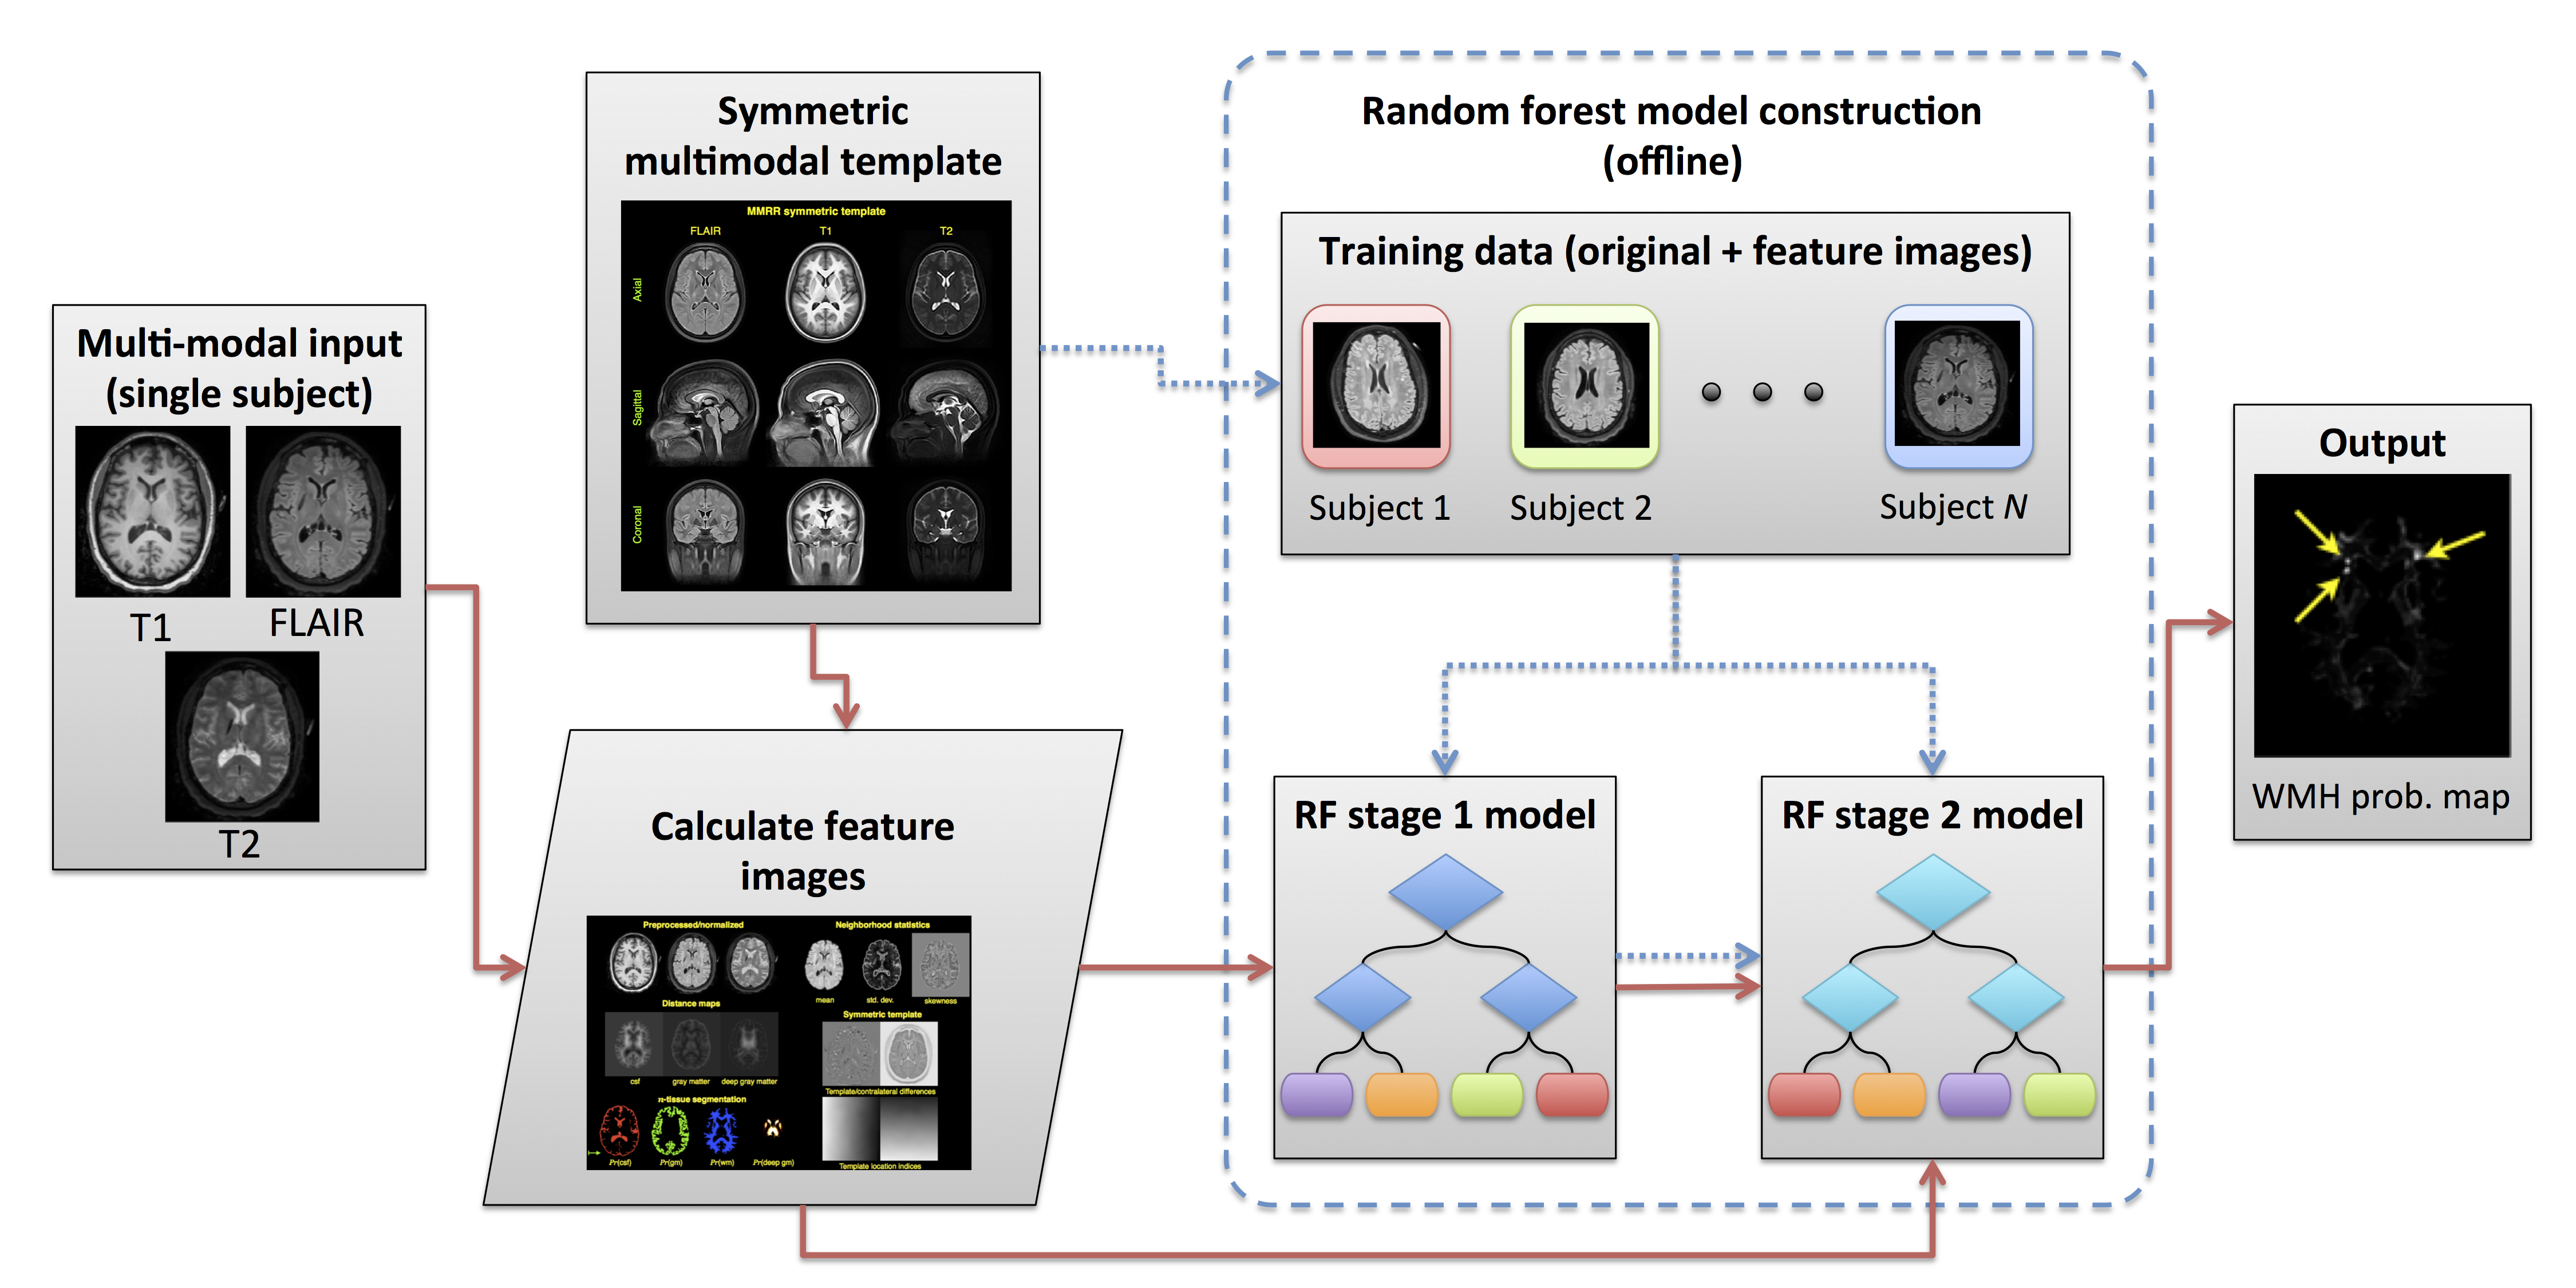
\includegraphics{Figures/wmhPipeline.png}
\caption{\textcolor{blue}{Workflow illustration for the proposed pipeline.  Processing of the multi-modal
input MRI for a single subject, using the multi-modal symmetric template, results in
the generation of the feature images.  These feature images are used as input to the
Stage 1 RF model producing the initial RF probability map estimates.  The Stage 1
voting maps, the original feature images, and the Stage 2 RF model result in the
final voting maps which includes the WMH probability estimate.  Note that the RF models
are constructed once from a set of training data which are processed using the
same feature-construction pipeline as the single-subject input MRI.}}
\end{figure}

\clearpage

\subsection*{References}\label{references}
\addcontentsline{toc}{subsection}{References}

\hypertarget{refs}{}
\hypertarget{ref-Avants:2014aa}{}
1. Avants BB, Tustison NJ, Stauffer M, Song G, Wu B, Gee JC. The Insight
ToolKit image registration framework. Front Neuroinform. 2014;8:44.

\hypertarget{ref-Yushkevich:2006aa}{}
2. Yushkevich PA, Piven J, Hazlett HC, Smith RG, Ho S, Gee JC, Gerig G.
User-guided 3D active contour segmentation of anatomical structures:
Significantly improved efficiency and reliability. Neuroimage.
2006;31(3):1116--28.

\hypertarget{ref-Tustison:2014ab}{}
3. Tustison NJ, Cook PA, Klein A, Song G, Das SR, Duda JT, Kandel BM,
Strien N van, Stone JR, Gee JC, et al. Large-scale evaluation of aNTs
and freeSurfer cortical thickness measurements. Neuroimage.
2014;99:166--79.

\hypertarget{ref-Tustison:2015aa}{}
4. Tustison NJ, Shrinidhi KL, Wintermark M, Durst CR, Kandel BM, Gee JC,
Grossman MC, Avants BB. Optimal symmetric multimodal templates and
concatenated random forests for supervised brain tumor segmentation
(simplified) with aNTsR. Neuroinformatics. 2015;13(2):209--25.

\hypertarget{ref-landman2011}{}
5. Landman BA, Huang AJ, Gifford A, Vikram DS, Lim IAL, Farrell JAD,
Bogovic JA, Hua J, Chen M, Jarso S, et al. Multi-parametric neuroimaging
reproducibility: A 3-T resource study. Neuroimage. 2011;54(4):2854--66.

\hypertarget{ref-Avants:2010aa}{}
6. Avants BB, Yushkevich P, Pluta J, Minkoff D, Korczykowski M, Detre J,
Gee JC. The optimal template effect in hippocampus studies of diseased
populations. Neuroimage. 2010;49(3):2457--66.

\hypertarget{ref-Avants:2011aa}{}
7. Avants BB, Tustison NJ, Wu J, Cook PA, Gee JC. An open source
multivariate framework for \(n\)-tissue segmentation with evaluation on
public data. Neuroinformatics. 2011;9(4):381--400.

\hypertarget{ref-schapire1990}{}
8. Schapire R. The strength of weak learnability. Machine Learning.
1990;5:197--227.

\hypertarget{ref-freund1997}{}
9. Freund Y, Schapire R. A decision-theoretic generalization of on-line
learning and an application to boosting. Journal of Computer and System
Sciences. 1997;55:119--139.

\hypertarget{ref-ho1995}{}
10. Ho TK. Random decision forests. In: Document analysis and
recognition, 1995., proceedings of the third international conference
on. Vol. 1. 1995. pp. 278--282 vol.1.

\hypertarget{ref-amit1997}{}
11. Amit Y, Geman D. Shape quantization and recognition with randomized
trees. Neural Computation. 1997;9:1545--1588.

\hypertarget{ref-breiman2001}{}
12. Breiman L. Random forests. In: Machine learning. 2001. pp. 5--32.

\hypertarget{ref-Moen:2014aa}{}
13. Moen KG, Brezova V, Skandsen T, Håberg AK, Folvik M, Vik A.
Traumatic axonal injury: The prognostic value of lesion load in corpus
callosum, brain stem, and thalamus in different magnetic resonance
imaging sequences. J Neurotrauma. 2014;31(17):1486--96.

\hypertarget{ref-Anbeek:2004aa}{}
14. Anbeek P, Vincken KL, Osch MJP van, Bisschops RHC, Grond J van der.
Probabilistic segmentation of white matter lesions in mR imaging.
Neuroimage. 2004;21(3):1037--44.

\hypertarget{ref-Tustison:2013ac}{}
15. Tustison NJ, Avants BB. Explicit B-spline regularization in
diffeomorphic image registration. Front Neuroinform. 2013;7:39.

\hypertarget{ref-Avants:2011ab}{}
16. Avants BB, Tustison NJ, Song G, Cook PA, Klein A, Gee JC. A
reproducible evaluation of ANTs similarity metric performance in brain
image registration. Neuroimage. 2011;54(3):2033--44.

\end{document}
